\documentclass[aspectratio=169]{beamer}

% Shared Beamer settings for Elements of AIML lectures (UPES).
% Keep this file free of \documentclass to allow reuse via \input.

% Allow lecture sources to use shared theme/assets without copying them into each lecture folder.
% NOTE: These paths are relative to `Unit-xx/Lecture-yy/latex/` (and `Lab/Experiment-xx/latex/`).
\makeatletter
\def\input@path{{../../../_shared/}{../../../_shared/UPES-Beamer-Theme/}}
\makeatother

\usetheme{UPES}
\setbeamertemplate{navigation symbols}{}

\usepackage{amsmath}
\usepackage{amssymb}
\usepackage{booktabs}
\usepackage{graphicx}
\usepackage{hyperref}
\usepackage{xcolor}
\usepackage{listings}

% Code listings (general-purpose).
\lstset{
  basicstyle=\ttfamily\small,
  keywordstyle=\color{blue},
  commentstyle=\color{gray},
  stringstyle=\color{teal},
  showstringspaces=false,
  columns=fullflexible,
  breaklines=true
}

\usepackage{tikz}
\usetikzlibrary{arrows.meta,positioning,shapes.geometric,calc}

% Per-slide source line (references shown on the slide itself).
\newcommand{\slidesources}[1]{%
  \vfill
  {\tiny\color{gray}\raggedright\sloppy\parbox{\linewidth}{Sources: #1}\par}%
}

% Unit-wise source strings for this subject (used by slides/notes).
% Path is relative to the lecture `latex/` folder (the compilation CWD).
% Source strings for Elements of AIML (used by slides + notes).

\newcommand{\AIMLRepoURL}{https://github.com/tali7c/Elements-of-AIML}

\newcommand{\AIMLLabSources}{%
Provost and Fawcett, \textit{Data Science for Business}.;%
McKinney, \textit{Python for Data Analysis}.;%
WEKA Documentation (Waikato Environment for Knowledge Analysis), accessed 2026-02-28.;%
Matplotlib and Seaborn documentation, accessed 2026-02-28.%
}

\newcommand{\AIMLUnitISources}{%
Rich and Knight, \textit{Artificial Intelligence}, McGraw Hill, 2017.;%
Russell and Norvig, \textit{Artificial Intelligence: A Modern Approach} (4e), Ch. 1--2 (Introduction, Intelligent Agents).;%
Poole and Mackworth, \textit{Artificial Intelligence: Foundations of Computational Agents} (2e), selected sections.%
}

\newcommand{\AIMLUnitIISources}{%
Russell and Norvig, \textit{Artificial Intelligence: A Modern Approach} (4e), Ch. 7--9 (Logical Agents, First-Order Logic, Inference).;%
Huth and Ryan, \textit{Logic in Computer Science} (2e), selected sections on propositional and first-order logic.;%
Genesereth and Nilsson, \textit{Logical Foundations of Artificial Intelligence}, selected chapters.%
}

\newcommand{\AIMLUnitIIISources}{%
Mueller and Massaron, \textit{Machine Learning for Dummies}, For Dummies, 2016.;%
Mitchell, \textit{Machine Learning}, selected chapters on learning basics and evaluation.;%
Scikit-learn documentation, accessed 2026-02-28.%
}

\newcommand{\AIMLUnitIVSources}{%
Mueller and Massaron, \textit{Machine Learning for Dummies}, For Dummies, 2016.;%
James, Witten, Hastie, and Tibshirani, \textit{An Introduction to Statistical Learning} (2e), selected chapters.;%
Scikit-learn documentation, accessed 2026-02-28.%
}

\newcommand{\AIMLUnitVSources}{%
NIST, \textit{AI Risk Management Framework (AI RMF 1.0)}, 2023.;%
Barocas, Hardt, and Narayanan, \textit{Fairness and Machine Learning} (online book), selected sections.;%
Knaflic, \textit{Storytelling with Data}, selected chapters on communicating results.%
}



\title[Elements of AIML]{Elements of AIML}
\subtitle{Unit 03 -- Lecture 01: Introduction to Machine Learning \& Datasets}
\author{Tofik Ali}
\institute{School of Computer Science, UPES Dehradun}
\date{\today}

\graphicspath{{../images/}{../../../_shared/}{../../../_shared/UPES-Beamer-Theme/}}

\begin{document}

\UPESCoverFrame
\setcounter{framenumber}{0}

\begin{frame}
  \titlepage
  \vspace{0.3em}
  \begin{center}
    \footnotesize Topic focus: \textbf{what it means to learn from data} + dataset basics\\[0.25em]
    \footnotesize Repository: \texttt{\AIMLRepoURL}
  \end{center}
  \slidesources{\AIMLUnitIIISources}
\end{frame}

\begin{frame}{Quick Links}
  \centering
  \hyperlink{sec:ml}{\beamerbutton{ML Basics}}\hspace{0.6em}
  \hyperlink{sec:data}{\beamerbutton{Datasets}}\hspace{0.6em}
  \hyperlink{sec:features}{\beamerbutton{Features}}\hspace{0.6em}
  \hyperlink{sec:example}{\beamerbutton{Example}}\hspace{0.6em}
  \hyperlink{sec:summary}{\beamerbutton{Summary}}
\end{frame}

\begin{frame}{Agenda}
  \tableofcontents
\end{frame}

\section{ML basics}
\label{sec:ml}

\begin{frame}{Learning Outcomes}
  By the end of this lecture, you should be able to:
  \begin{itemize}[<+->]
    \item Define \textbf{machine learning} and describe common task types.
    \item Explain what a \textbf{dataset} is (rows, columns, features, labels).
    \item Distinguish \textbf{features} vs \textbf{labels} and list common data types.
    \item Identify basic data issues (missing values, outliers, noise) that affect ML.
  \end{itemize}
\end{frame}

\begin{frame}{Abbreviations \& Symbols}
  \begin{itemize}[<+->]
    \item ML: Machine Learning \hfill EDA: Exploratory Data Analysis
    \item $X$: feature matrix \hfill $y$: label/target vector
    \item $n$: number of examples (rows) \hfill $d$: number of features (columns)
    \item $K$: number of classes (classification) \hfill $\hat{y}$: prediction
    \item $f(\cdot)$: model/function learned from data
  \end{itemize}
\end{frame}

\begin{frame}{What is Machine Learning?}
  \begin{block}{Informal definition}
    ML is about building models that \textbf{learn patterns from data} to make predictions or decisions.
  \end{block}
  \vspace{0.4em}
  \begin{itemize}[<+->]
    \item Instead of writing rules manually, we learn a function from examples.
    \item Learning requires: data, an objective, and a way to evaluate performance.
  \end{itemize}
\end{frame}

\begin{frame}{A Standard Definition (Mitchell)}
  A program learns from \textbf{experience} $E$ with respect to some \textbf{task} $T$ and \textbf{performance measure} $P$ if its performance at $T$, as measured by $P$, improves with $E$.
  \vspace{0.5em}
  \begin{exampleblock}{Example (spam detection)}
    $T$: classify email as spam/ham,\; $E$: labeled emails,\; $P$: accuracy/F1 on unseen emails.
  \end{exampleblock}
\end{frame}

\begin{frame}{ML Workflow (Big Picture)}
  \centering
  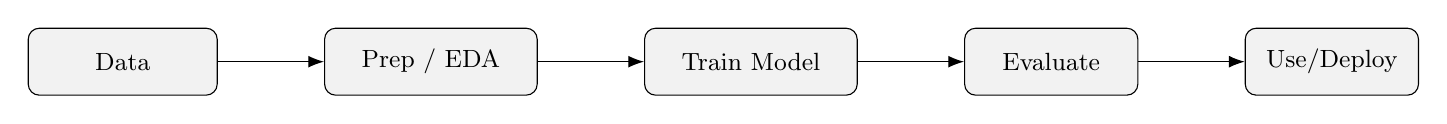
\begin{tikzpicture}[node distance=1.35cm, every node/.style={font=\small}]
    \node (data) [draw, rounded corners, fill=gray!10, minimum width=2.4cm, minimum height=0.85cm] {Data};
    \node (prep) [draw, rounded corners, right=of data, fill=gray!10, minimum width=2.7cm, minimum height=0.85cm] {Prep / EDA};
    \node (train) [draw, rounded corners, right=of prep, fill=gray!10, minimum width=2.7cm, minimum height=0.85cm] {Train Model};
    \node (eval) [draw, rounded corners, right=of train, fill=gray!10, minimum width=2.2cm, minimum height=0.85cm] {Evaluate};
    \node (use)  [draw, rounded corners, right=of eval, fill=gray!10, minimum width=2.2cm, minimum height=0.85cm] {Use/Deploy};
    \draw[-{Latex[length=2mm]}] (data) -- (prep);
    \draw[-{Latex[length=2mm]}] (prep) -- (train);
    \draw[-{Latex[length=2mm]}] (train) -- (eval);
    \draw[-{Latex[length=2mm]}] (eval) -- (use);
  \end{tikzpicture}
  \vspace{0.4em}
  \small Key idea: evaluation must reflect the \textbf{future/unseen} setting.
\end{frame}

\begin{frame}{Common ML Task Types}
  \begin{itemize}[<+->]
    \item \textbf{Supervised learning}: learn from labeled data
      \begin{itemize}
        \item regression (predict a number), classification (predict a class)
      \end{itemize}
    \item \textbf{Unsupervised learning}: learn structure without labels
      \begin{itemize}
        \item clustering, dimensionality reduction
      \end{itemize}
    \item \textbf{Reinforcement learning}: learn via rewards from interaction (Unit IV overview)
  \end{itemize}
\end{frame}

\begin{frame}{Tasks at a Glance (What changes?)}
  \centering
  \begin{tabular}{lll}
    \toprule
    \textbf{Task} & \textbf{Input} & \textbf{Output} \\
    \midrule
    Regression & $x$ features & number (e.g., price) \\
    Classification & $x$ features & class (e.g., spam/ham) \\
    Clustering & $x$ only & group/cluster id \\
    Dim. reduction & $x$ only & lower-dim representation $z$ \\
    \bottomrule
  \end{tabular}
  \vspace{0.5em}
  \small Same dataset can support multiple tasks depending on the objective.
\end{frame}

\section{Datasets}
\label{sec:data}

\begin{frame}{Dataset View (Tabular)}
  \begin{itemize}[<+->]
    \item Many ML problems use a table: \textbf{rows} are examples, \textbf{columns} are variables.
    \item Inputs are \textbf{features} ($X$), output is \textbf{label/target} ($y$).
    \item Goal: learn a mapping $f: X \rightarrow y$ that generalizes.
  \end{itemize}
\end{frame}

\begin{frame}{Dataset Notation (Typical)}
  \begin{itemize}[<+->]
    \item Feature matrix:
    \[
      X \in \mathbb{R}^{n \times d}
    \]
    \item Regression target:
    \[
      y \in \mathbb{R}^{n}
    \]
    \item Classification target:
    \[
      y \in \{1,\dots,K\}^{n}
    \]
  \end{itemize}
  \vspace{0.2em}
  \small $n$ = samples, $d$ = features, $K$ = classes.
\end{frame}

\begin{frame}{Data Types You Will See}
  \begin{itemize}[<+->]
    \item \textbf{Numerical}: integers, floats (e.g., age, income)
    \item \textbf{Categorical}: finite set of values (e.g., city, department)
    \item \textbf{Ordinal}: ordered categories (e.g., low/medium/high)
    \item \textbf{Text / images / time series}: require feature representations
  \end{itemize}
\end{frame}

\section{Feature sets}
\label{sec:features}

\begin{frame}{Features: The Representation Matters}
  \begin{itemize}[<+->]
    \item A \textbf{feature} is a measurable property used by a model.
    \item Good features make learning easier; bad features can make any model fail.
    \item Feature sets often require:
      \begin{itemize}
        \item encoding (e.g., one-hot), scaling, cleaning, transformations
      \end{itemize}
  \end{itemize}
\end{frame}

\begin{frame}{From Raw Data to Features (Examples)}
  \begin{itemize}[<+->]
    \item Raw text $\rightarrow$ word counts / TF-IDF / embeddings
    \item City name (categorical) $\rightarrow$ one-hot encoding
    \item Time stamp $\rightarrow$ hour-of-day, day-of-week, seasonality features
    \item Image $\rightarrow$ pixel values or learned features (CNN)
  \end{itemize}
  \vspace{0.3em}
  \small The model only ``sees'' the feature representation you provide.
\end{frame}

\begin{frame}{Common Data Problems (Preview to Labs)}
  \begin{itemize}[<+->]
    \item Missing values (NaN): require imputation or removal
    \item Outliers: can distort averages and some models
    \item Duplicates and inconsistent formatting
    \item Noisy labels: incorrect ground truth
  \end{itemize}
  \vspace{0.4em}
  These issues are the focus of the lab experiments on EDA and preprocessing.
\end{frame}

\section{Mini example}
\label{sec:example}

\begin{frame}{Example: House Price Prediction}
  \begin{itemize}[<+->]
    \item Goal: predict price (target $y$)
    \item Features ($X$): area, number of rooms, location, age of house
    \item Regression model learns: $Price \approx f(Area, Rooms, Location, Age)$
  \end{itemize}
  \vspace{0.4em}
  Question: what if \textbf{location} is categorical? $\rightarrow$ we must encode it.
\end{frame}

\begin{frame}{Mini Worked Example (Tiny Dataset)}
  \centering
  \begin{tabular}{lrrr}
    \toprule
    Location & Area & Rooms & Price \\
    \midrule
    A & 1200 & 2 & 55 \\
    B & 1500 & 3 & 72 \\
    A & 900  & 2 & 48 \\
    \bottomrule
  \end{tabular}
  \vspace{0.4em}
  \small To use \textbf{Location}, encode it (e.g., one-hot) instead of treating A/B as numeric.
\end{frame}

\section{Summary}
\label{sec:summary}

\begin{frame}{Summary}
  \begin{itemize}
    \item ML learns a mapping from data; supervised vs unsupervised vs RL.
    \item Datasets contain examples (rows) and variables (columns).
    \item Features are representations; data quality strongly affects results.
    \item Next: train/test/validation splits and cross-validation (Lecture 02).
  \end{itemize}
  \slidesources{\AIMLUnitIIISources}
\end{frame}

\begin{frame}{Exit Questions}
  \begin{enumerate}
    \item Define machine learning in your own words.
    \item What is the difference between features and labels?
    \item Give two examples each of supervised and unsupervised tasks.
    \item Name three common dataset issues that affect model performance.
  \end{enumerate}
\end{frame}

\end{document}
